\documentclass[border=3mm,tikz,preview]{standalone}
\usepackage[utf8]{inputenc}
\usepackage{amsmath,amssymb,amsfonts}
\usepackage{graphicx}
\usepackage{tikz}
\usetikzlibrary{shapes.geometric, arrows.meta, positioning, shadows, calc, fit, backgrounds}
\usepackage{xcolor}
\begin{document}

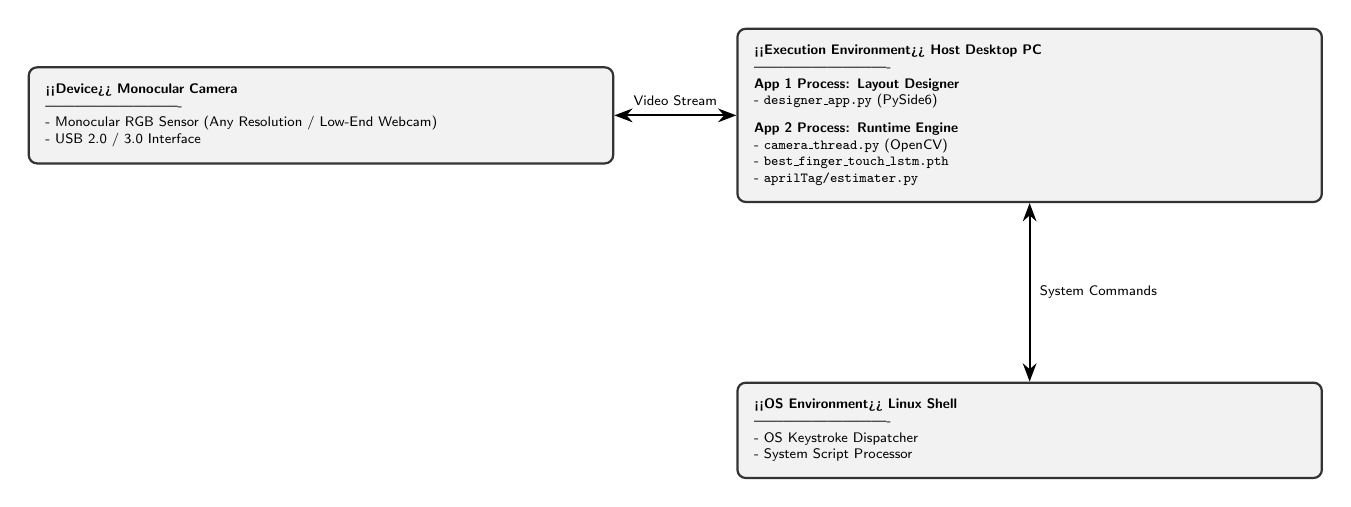
\begin{tikzpicture}[
    nodebox/.style = {rectangle, draw=black!80, fill=gray!10!white, thick, rounded corners=3pt, align=left, font=\sffamily\tiny, inner sep=6pt, text width=7cm},
    conn/.style = {draw=black, thick, <->, >=Stealth}
]

% Nodes
\node (n_cam) [nodebox] at (0,0) {
\textbf{<<Device>> Monocular Camera}\\
----------------------------\\
- Monocular RGB Sensor (Any Resolution / Low-End Webcam)\\
- USB 2.0 / 3.0 Interface
};

\node (n_host) [nodebox] at (9,0) {
\textbf{<<Execution Environment>> Host Desktop PC}\\
----------------------------\\
\textbf{App 1 Process: Layout Designer}\\
- \texttt{designer\_app.py} (PySide6)\\[4pt]
\textbf{App 2 Process: Runtime Engine}\\
- \texttt{camera\_thread.py} (OpenCV)\\
- \texttt{best\_finger\_touch\_lstm.pth}\\
- \texttt{aprilTag/estimater.py}
};

\node (n_os) [nodebox] at (9,-4) {
\textbf{<<OS Environment>> Linux Shell}\\
----------------------------\\
- OS Keystroke Dispatcher\\
- System Script Processor
};

% Connections
\draw [conn] (n_cam) -- node[above, font=\sffamily\tiny]{Video Stream} (n_host);
\draw [conn] (n_host) -- node[right, font=\sffamily\tiny]{System Commands} (n_os);

\end{tikzpicture}

\end{document}
